\chapter{Modular design: Concepts, methods, and applications in engineering, biology, and biotechnology}\label{ch:review}
% (Review paper)


\disclose{Modular design: Implementing proven engineering principles in biotechnology. Garcia, S., and Trinh, C. T. Biotechnology Advances, 2019}%{garcia2019b}

%\textbf{Modular design: Implementing proven engineering principles in
%biotechnology}

%Sergio Garcia\textsuperscript{1,2} and Cong T.
%Trinh\textsuperscript{1,2,}*
%\textsuperscript{1}Department of Chemical and Biomolecular Engineering,
%University of Tennessee, Knoxville, Tennessee
%
%\textsuperscript{2}Center for Bioenergy Innovation, Oak Ridge National
%Laboratory, Oak Ridge, Tennessee
%
%%*Corresponding author: \href{mailto:ctrinh@utk.edu}{\nolinkurl{ctrinh@utk.edu}}
%\hypertarget{abstract}{%
%\section{\texorpdfstring{\\
%\textbf{Abstract}}{ Abstract}}\label{abstract}}

\section*{Abstract}

Modular design is at the foundation of contemporary engineering, enabling rapid, efficient, and reproducible construction and maintenance of complex systems across applications.
Remarkably, modularity has recently been discovered as a governing principle in natural biological systems from genes to proteins to complex networks within a cell and organism communities.
The convergent knowledge of natural and engineered modular systems provides a key to drive modern biotechnology to address emergent challenges associated with health, food, energy, and the environment.
Here, we first present the theory and application of modular design in traditional engineering fields.
We then discuss the significance and impact of modular architectures on systems biology and biotechnology.
Next, we focus on the very recent theoretical and experimental advances in modular cell engineering that seeks to enable rapid and systematic development of microbial catalysts capable of efficiently synthesizing a large space of useful chemicals.
We conclude with an outlook towards theoretical and practical opportunities for a more systematic and effective application of modular engineering in biotechnology.

%\textbf{Key words:} Modular design; modularity; modular cell; modular
%cell engineering; ModCell; systems biology; metabolic engineering;
%synthetic biology; robustness; evolvability; networks; Pareto
%optimality; industrialization of biology; microbial biocatalysis.


\section{Introduction}

Complex engineered systems such as computers, vehicles, or factories can be assembled from exchangeable units of self-contained functionality known as modules.
Modular design enables efficient production, maintenance, and customization across modern engineering technologies.
The inception of modular design has had a revolutionary impact on many industries.
For instance, the first modular computer, named IBM System/360 and built in the 1960s, allowed to use the same software for different application-dependent hardware, shaping information technology as we know it today.\citep{o2018}
Undoubtedly, modular design will continue to drive innovation in both established and emergent fields of engineering.

Among trending engineering disciplines, biotechnology is encompassing far-reaching applications driven by the recent development of enabling technologies in interdisciplinary areas of genome engineering \citep{barrangou2016}, systems and synthetic biology \citep{kahl2013}.
metabolic engineering \citep{nielsen2016}, and bioprocessing \citep{cramer2011, olson2012}.
Amid many applications to address issues related to health, energy, and the environment, the chemical industry will benefit from metabolic reprogramming of microbes as cell factories to catalyze the synthesis of therapeutics, chemicals, and fuels, from renewable and sustainable feedstocks (e.g., lignocellulosic biomass, sugar cane) or waste products (e.g., waste gas from steel manufacturing, plastic waste).
Even though there exists a naturally large space of molecules that can be synthesized by metabolically engineered microorganisms \citep{lee2019}, fewer than a dozen molecules are industrially produced \citep{nielsen2016}.
A major roadblock is attributed to the very laborious and costly strain engineering process partly arising from the lack of standardization and repetition of genetic manipulation tasks \citep{king2017, winkler2015}.
Recently, modular cell engineering has been proposed as an innovative approach to accelerate strain engineering process, harnessing a large space of molecules derived from rich and diverse cellular metabolism and thus pushing whole-cell biocatalysis towards an industrially competitive technology \citep{trinh2016}.

In this paper, we first examine the theory and application of modular design in conventional engineering disciplines, such as mechanical, chemical, nuclear, and civil engineering, with the aim to provide perspectives and innovative methods that can be transferred to biotechnology.
We next present the importance of modularity that exists in natural biological systems.
Finally, we highlight the most recent theoretical and experimental developments in modular cell design for synthetic biology and metabolic engineering applications.

\section{Modularity in engineered systems}

\subsection{Basic concepts}

Based on the definition by Miller and Elgard \citep{miller1998}, a module is "an essential and self-contained functional unit relative to the product of which it is part.
The module has, relative to a system definition, standardized interfaces and interactions that allow composition of products by combination".
We find this definition, out of the many available \citep{salvador2007}, to be general yet descriptive enough to illustrate the topics in this paper.
Based on the above definition, modules must have a standardized interface and exchangeability in order to enable rapid and systematic assembly of components into a system with various types of modular architectures \citep{ulrich1995}.
A fully modular or sectional architecture has all the components to be modules, for instance, fluid pipes or sectional couches, while an integral architecture lacks any type of modules (Figure~\ref{fig:ba-fig1}~A).
Chassis-based architectures are also common in modular design, including bus and slot.
The bus modular architecture uses the same interface for all modules, e.g., universal serial bus (USB) and peripheral component interconnect (PCI) ports found in computers, while the slot modular architecture has specific interfaces for corresponding modules, e.g., tires in an automobile.
The chassis-based architectures enable the use of alternative chasses that can be combined with the same modules to efficiently generate a variety of products or vice versa \citep{jose2005}.


\subsection{Driving forces and potential tradeoffs of modular design}

The driving forces for system modularization are to achieve increased efficiency and robustness, reduced complexity and cost, and better customization and maintenance options \citep{bonvoisin2016, miller1998}.
Modular design has been the core of many innovative technologies across engineering disciplines (Figure~\ref{fig:ba-fig1}~B).
For instance, modularized plants in chemical engineering allow faster and more cost-effective deployment, making small operations viable and hence providing economic and environmental advantages \citep{baldea2017, kim2017}.
Likewise, modular buildings in civil engineering enable more rapid and economical construction \citep{kamali2016}.
In nuclear engineering, the use of small modularized reactors overcomes potential hazards of traditional large-scale operations, allows plant customization to energetic demand, and reduces construction and manufacturing costs \citep{RN137}.
The emerging area of highly automated manufacturing also implements modular production systems \citep{weyer2015}.
In addition, modular design principles have been applied with great success in abstract engineering disciplines such as software \citep{abelson1996, gancarz2003} and management engineering \citep{campagnolo2010}.
The decomposition of software elements into modules of defined functionality is essential to manage complexity, ensure robustness, and allow for concurrent development.
Similarly, organizations and projects can be structured into modules to accomplish parallel task execution and avoid repetition.

Even though modular design is ubiquitous, it may not be desirable or feasible in every circumstance.
The disadvantages and limitations of modularity tend to be field specific.
When modularity is part of an innovative approach, such as modular chemical plants, a lack of experience and higher upfront costs are regarded as common drawbacks \citep{baldea2017}.
Design constraints may also limit the applicability of modularity; for example, a quantitative study \citep{RN26} suggested that the portability requirements of cell phones and laptops makes them less modular than their static counterparts.
In the case of buildings and chemical plants, the size of components may prevent off-site modular manufacturing if transportation is unfeasible.
Thus, when choosing modular design for engineering applications, it is important to ensure that advantages outweigh disadvantages.

\subsection{Theoretical frameworks of modular design}

Modular product design is complex and field-specific but can be generally formulated using the language of graph theory.
The Design Structure Matrix (DSM) \citep{browning2016} is a commonly used technique to model a system as a graph, where nodes represent basic components and links between nodes describe their functional interactions.
Component interactions can be represented in a binary manner (i.e., whether a relationship exists or not) or in a detailed complex fashion with multiple dimensions and values to increase model accuracy.
For example, with a complex interaction, a metric can be used to quantitatively assign interaction desirability between two components, i.e., a high desirability score if they require each other to work or a negative desirability score otherwise.
In some cases, detailed interaction types can also be classified and integrated in the modular design; for example, a cooling system with a radiator and a fan is required to have not only a \emph{spatial} interaction (i.e., both elements need to be in close proximity) but also a \emph{material} interaction (i.e., the fan provides airflow across the radiator) (Figure~\ref{fig:ba-fig1}~ C) \citep{helmer2010}.

DSM can reveal properties of the system through different analyses, including singular value decomposition to capture the modular architecture type (e.g.
integral, chassis-based, bus, or slot) \citep{RN26}, node centrality ranking to identify key interactions between modules and interfaces \citep{sosa2007}, and most importantly, clustering to identify modules (Figure~\ref{fig:ba-fig1}~ C).
While many approaches exist to cluster a DSM, not all can successfully identify modules due to underlying design conflicts in product modularization; for these scenarios, integrated use of a highly descriptive DSM model to account for complex interactions and multi-objective optimization to identify Pareto optimal solutions is needed to accurately design modular systems \citep{helmer2010}.

\section{Modularity in biological systems}

In the high-throughput and quantitative era of biology, modularity has become a fundamental abstraction in understanding and redesigning biological systems that have existed and evolved for billions of years \citep{hartwell1999, wagner2007}.
A variety of definitions of biological modules co-exist, arising from the multi-scale and multi-interaction nature of biological systems.
From a mathematical perspective, two general approaches are commonly used to define modules: (i) modules as clusters of highly interconnected nodes in a biological interaction network, and (ii) modules as programmable circuits that can be described with laws of mass and energy conservation and control theory.
These paradigms differ in that network modules provide a holistic and simplified description, while circuit modules provide a reductionistic and detailed description.
Despite their differences, both approaches seek to understand the evolutionary origin of modules, their role in fundamental biological properties such as robustness and evolvability, and their biotechnological applications.

\subsection{Modularity exists across all scales of biology}

Modularity is a ubiquitous organizing principle across all scales of biology.
Within a scale, modules often interact in a hierarchical manner (Figure~\ref{fig:ba-fig2}).
At the molecular level, DNA transcription activation and rate can be controlled by a variety of modular promoter elements \citep{dynan1989}.
Additionally, certain proteins are highly modular, such as enzymes (e.g., polyketide synthase and non-ribosomal peptide synthetase \citep{hutchinson2003}) with modular substrate identification elements that enable biosynthesis of a large space of secondary metabolites \citep{khosla2001}.
At the cellular level, modularity is present in all biomolecule interaction networks \citep{mitra2013}, including RNAs \citep{stuart2003}, proteins \citep{spirin2003}, and metabolites \citep{ravasz2002}.
In all cases, modules are associated with specific cellular functions or pathways, which often interact in a hierarchical manner \citep{ravasz2002}.
At the multi-cellular level, organs and tissues are also structured modularly.
For example, in the human brain, neuron interaction networks contain modules associated with specific cognitive functions \citep{sporns2016}.
These modules are hierarchically organized into submodules to integrate and contextualize specialized functions of the brain \citep{meunier2010}; for instance, visual perception that requires the functional integration of multiple neuron clusters in the cortical columns \citep{park2013}.
At the ecological scale, organism communities can be represented by networks, where nodes are species or subpopulations and links are interactions such as consumption, pollination, or competition \citep{grilli2016}.
The capability of ecological networks to avoid global failure due to small perturbations has been attributed to their modular structure both theoretically \citep{grilli2016} and experimentally \citep{gilarranz2017}.

\subsection{Modularity explains functions of components and interactions of biological systems}

Prior to the systems biology era, the view of modular biological systems can be traced back as early as the late 19\textsuperscript{th} century with the initial study of what later became known as glycolysis to investigate how yeast fermentation made wine have a good taste.
Throughout the first half of the 20\textsuperscript{th} century, the complete knowledge of many major metabolic pathways of well-defined functionality across organisms, including the EMP pathway, the Entner-Doudoroff pathway, Krebs cycle, pentose phosphate pathway, and so on, was established.
These pathways were mapped to qualitatively describe the modular interconnection of functional elements within a cell, i.e., cellular metabolism that governs cell physiology.
Pioneering work in the 1980s, including the comprehensive description of measurable bacterial cellular components \citep{neidhardt1990} and constraint-based simulations of microbial metabolism \citep{fell1986}, helped establish a foundation for quantitative modular analysis of cell physiology.
With the explosion of high-throughput `omics technologies in the late 90's, complex biological systems with thousands of interacting elements can now be studied holistically and quantitatively at multiple levels from genes to proteins and metabolites within the cell and microbial communities \citep{rodriguez2014, lowe2017, patti2012, wilkins1996}.
Graphs (or networks) can represent these systems \citep{alon2003} and their complex interactions, e.g., metabolites-enzymes \citep{ma2003, ravasz2002}, genes-diseases \citep{goh2007}, protein-protein \citep{szklarczyk2017}, or a combination of all known protein and genetic interactions \citep{chatr-aryamontri2017}.
Module analysis of biological networks can provide two insights: (i) identification of modules that represent transferable and self-contained functions \citep{mitra2013}, for example, a cis-regulatory element and its associated genes \citep{ohta2008}, the subunits of a protein complex \citep{guruharsha2011, havugimana2012}, and the genes associated with a disease phenotype \citep{goh2007}, and (ii) interactions among modules of a system.
For example, by analyzing the metabolic networks of 43 organisms, Ravasz \emph{et al.} \citep{ravasz2002} identified a hierarchical modular architecture containing hubs of highly connected metabolites and modules with specific metabolic functions.
Remarkably, the identified architecture overlaps with the known primary and secondary metabolic pathways.
Likewise, by analyzing metabolic networks of 63 organisms, Ma and Zeng \citep{ma2003} could identify a bow-tie architecture of the network containing a core of highly interconnected components linking input and output node clusters.
Graph-based analysis of metabolic networks also revealed a small-world architecture (i.e., a small number of reactions between any two metabolites) that was hypothesized to confer cellular metabolism with the capability to quickly adapt to perturbations \citep{wagner2001}.

\subsection{Modularity is a foundational tool to control programmable cells}

Genetic circuits are modules that define a universal programming language of cells, such as logical gates \citep{brophy2014, nielsen2016}, and can be widely found in natural biological systems.
Classical examples of genetic circuits are the lac operon that enables carbon catabolite repression in bacteria and the MAPK/ERK signaling pathway in mammalian cells that controls cell division among other cellular functions.
Modularity of natural signaling pathways can be harnessed for novel functions \citep{lim2010, pryciak2009}, including the production of valuable metabolites, synthesis of nanomaterials, treatment of disease, and sensors to detect hazardous molecules \citep{brophy2014}.
The laws of mass and energy conservation and principles of control theory that have been well developed in traditional engineering disciplines can be applied to enable modular design of synthetic biological systems.
For instance, Del Vecchio \emph{et al.} \citep{del2008} developed a mathematical model of retroactivity that captures the impact of a downstream module on the function of an upstream module, and used this model to enhance module insulation.
Even though synthetic genetic circuit modules operate correctly and reliably in an isolated environment, it remains challenging to integrate these modules into complex systems \citep{purnick2009}.

\subsection{Modularity enables evolutionary advantage and robustness}

Biological robustness is the ability of a system to maintain its function upon genetic and environmental perturbations.
Both the graph- and circuit-based descriptions of modules \citep{whitacre2012} can help explain their contributions to system robustness.
For example, the bow-tie architecture of biological networks \citep{friedlander2015} has been suggested \citep{kitano2004} to enhance the biological robustness of chassis-based modularity, where the essential core processes belong to the conserved chassis and adaptable modules allow for evolution to experiment safely.
This view, however, raises the question of the evolutionary origin and function of modules.
It has been hypothesized that modules may arise due to natural selection or biased mutational mechanisms.
Computational studies on the topic are abundant but compatible with both hypotheses \citep{wagner2007}.
Several models have suggested that when a single fitness goal is present, a modular architecture does not emerge since it does not provide a fitness advantage.
However, when multiple fitness goals are pursued, either sequentially \citep{kashtan2007} or simultaneously \citep{clune2013}, a modular architecture is favored.
Additionally, it has been demonstrated that macroscopic \citep{shoval2012} and molecular \citep{schuetz2012} phenotypes are weighted combinations of optimal phenotypes specialized for single tasks.
This view is important in the context of modular cell engineering that can be formulated as a multi-objective optimization problem \citep{garcia2019}, where each fitness goal corresponds to a module for making a desirable chemical.
Thus, modular cell engineering can harness the existing features of biological modularity instead of creating entirely synthetic properties.

\section{Modular cell engineering}

Diverse and complex cellular metabolism encompasses a large space of molecules, providing a potential path towards broader industrialization of biology \citep{connelly2015}.
To realize this potential, rapid development of novel microbial biocatalysts to efficiently synthesize these molecules is critical but faces multiple challenges due to laborious and costly requirement of extensive strain optimization cycles \citep{nielsen2016, trinh2016}.
Effective exploitation of modular design as seen in natural and engineered systems for biocatalyst development can offer innovative strategies to tackle these challenges.

To date, modular cell engineering has been mostly applied at the pathway level, where enzyme module expression is adjusted to increase target metabolite production.
This topic has been extensively reviewed \citep{biggs2014, jeschek2017, lu2018, yadav2012} and will not be elaborated in detail here.
At the cellular level, platform strains engineered to eliminate common byproducts and increase availability of important precursors for overproduction of target molecules have been reported with some success by implementing the conventional ``push-and-pull'' metabolic engineering strategy \citep{nielsen2016}.
More recently, a system-level modular cell design method has been developed to systematically and simultaneously design both the chassis cell and production modules for the synthesis of various target chemicals \citep{garcia2019, trinh2015}.
Unlike conventional strain optimization methods that target one product, modular cell design seeks to enable rapid and predictable creation of multiple production strains to achieve superior performance with minimal strain optimization cycle where each synthesizes a different product.
Each optimal production strain is obtained by assembling a reusable modular (chassis) cell with an exchangeable production module(s) in a plug-and-play fashion, resembling the advantages of modular design in traditional engineering disciplines.
Specifically, a modular cell contains core metabolic phenotypes shared among production modules (Figure~\ref{fig:ba-fig3}~A).
The chassis interfaces with the modules through enzyme synthesis machinery and precursor metabolites (Figure~\ref{fig:ba-fig3}~B).
Modules contain auxiliary regulatory and metabolic pathways (Figure~\ref{fig:ba-fig3}~C) that enable a desired phenotype for optimal biosynthesis of a target molecule, such as growth-coupled-to-product formation (\emph{GCP} design) or stationary-phase product synthesis (\emph{NGP} design) (Figure~\ref{fig:ba-fig3}~D).
These design principles are formulated to integrate state-of-the-art techniques developed in the fields of synthetic biology and metabolic engineering, including, (1) computational models that identify genetic interventions towards desirable phenotypes, (2) rapid discovery and optimization of metabolic pathways for target product synthesis (i.e., production modules), and (3) design of minimal cells and orthogonal pathways to generate a toolkit of parts that can be assembled into various functional systems.

In the following sections, we highlight the recent advancements in modular cell engineering that capture: (1) design principles and computational tools to enable construction of a modular cell and associated production modules, (2) discovery and optimization of metabolic pathways as production modules both theoretically and experimentally, and (3) experimental implementation of modular cell design principles.

\subsection{Recent developments in mathematical formulation of modular cell design}


The primer for the modular cell design principles started with the observation \citep{trinh2012} that the optimal design of the n-butanol- and isobutanol-producing \emph{E.
coli} cells\emph{,} based on constraint-based modeling \citep{palsson2015} and conventional strain design methods \citep{trinh2009}, exhibited the same core metabolism (Figure~\ref{fig:ba-fig4}~A-B).
To systematically explore this property, the first modular cell design method, called MODCELL, was proposed and used to design an \emph{E.
coli} modular cell for alcohol and ester production \citep{trinh2015} (Figure~\ref{fig:ba-fig4}~E).
In Chapter~\ref{ch:ms1} a new formulation of the modular cell design problem, ModCell2, based on multi-objective optimization will be developed to design strains with minimal trade-off between compatibility, performance, and robustness (Figure~\ref{fig:ba-fig4}~H).

%A new formulation of the modular cell design problem, ModCell2 \citep{garcia2019}, was proposed based on the framework of multi-objective optimization to capture the tradeoffs that may exist among highly diverse biochemical pathways.
%ModCell2 enables analysis of genome-scale metabolic networks with many production modules and design of optimal modules without extensive prior knowledge of target pathways.
%ModCell2 was used to demonstrate that a modular cell can be designed to exhibit (i) desirable production phenotypes for many molecules under various culturing conditions beyond the growth-coupled to product synthesis phase \citep{klamt2015}, such as the stationary-phase phase \citep{klamt2018}, and (ii) minimal trade-off between compatibility, performance, and robustness (Figure~\ref{fig:ba-fig4}~H).
%These results highlight that the systems-level modularization of cellular metabolism can accelerate strain engineering without sacrificing performance requirements.

While ModCell2 is to our knowledge the only tool that involves simultaneous design of chassis, modules, and interfaces, other recently developed computational tools can be applied to design these elements individually.
For example, MinGenome \citep{wang2018} is used to design genomes of minimal cells that can serve as chassis whereas ValveFind \citep{pandit2017} enables design of orthogonal pathways to build production modules.
Topics on model-guided strain design techniques for ``integral'' strains, .i.e, strains optimized for production of only a single product, can be found in recent excellent reviews.
\citep{long2015, machado2015, ng2015}.

Future development of modular cell design tools will incorporate enzyme kinetics of cellular metabolism \citep{king2015, noor2016} to account for potential metabolic burdens \citep{wu2016} in the design of modular cells and exchangeable production modules (Figure~\ref{fig:ba-fig4}~I).
Enzyme cost analysis is also particularly useful for identifying robust strategies for adaptive laboratory evolution that prevent an unintended pathway(s) to be optimized instead of a targeted pathway(s) \citep{dinh2018}.
The lack of experimental data on enzyme catalytic efficiencies needed for these modeling approaches can be addressed through random parameter sampling \citep{dinh2018}, \emph{omics} integration \citep{ebrahim2016, khodayari2016}, and machine learning \citep{heckmann2018}.
Recently developed models that predict \emph{in-vivo} enzyme concentrations from the genetic sequence help bridge the gap between metabolic model predictions and experimental implementation \citep{farasat2014, meng2013, salis2009}.

\subsection{Recent advances in discovery and optimization of metabolic pathways as production modules}

With the arrival of quantitative `omics era in mid 1990s, we started to gain a deeper understanding of complex biological systems and categorize them into the functional biological parts, i.e., regulatory and functional genes for retrieval through development of biological databases (e.g., Registry of Standard Biological Parts (https://parts.igem.org), KEGG \citep{kanehisa2000}, Biocyc \citep{caspi2013}, Brenda \citep{scheer2010}, among many others).
Synergistically, the interdisciplinary areas of bioinformatics, synthetic biology, metabolic and protein engineering have also emerged, advanced, and now enabled rapid and systematic identification and assembly of these biological parts into production modules to probe a large space of molecules that are only limited by one's imagination.
Nowadays, development of production modules can start by using computational tools with increasing scope and accuracy \citep{kumar2018, wang2017}, that help identify metabolic steps, associated enzymes, and genetic parts (i.e., promoters, terminators, ribosome binding sites, regulatory/sensory elements, and so on) using a combination of elementary reaction rules, yield, thermodynamic, and biophysical analyses \citep{dugar2011, kumar2018}.
Next, the genetic parts can be synthesized, assembled, and characterized for accuracy in a rapid manner to build production modules to make desirable molecules in a target host \citep{annaluru2014, bitinaite2007, blake2010, chen2013, colloms2014, gibson2009, kok2014, li2005, li2007, shao2009, trubitsyna2014, tsuge2003, zhang2012b}.
Some recent achievements, highlighting innovations in retrofitting cellular metabolism for novel biocatalysis from sustainable feedstocks, include: (i) redirection of central metabolism to make environmentally friendly, non-natural bioplastics \citep{rehm2010}, (ii) redesign of fermentative pathways to produce a large space of designer bioesters used as flavors, fragrances, biofuels, and solvents \citep{layton2014, rodriguez2014} (Figure~\ref{fig:ba-fig4}~D), (iii) repurposing of the beta-oxidation pathway for combinatorial biosynthesis of alcohols, dicarboxylic acids, hydroxyl acids, and lactones as industrial platform chemicals \citep{cheong2016} (Figure~\ref{fig:ba-fig4}~F), and (iv) refactoring of polyketide and isoprenoid pathways to explore a large space of secondary metabolites as drugs \citep{ajikumar2010, galanie2015, martin2003}.

While the design, construction, and characterization of production modules can be streamlined, compatibility between the modules and a target host has always posed a significant challenge mainly due to the intricate flux imbalance resulting in low product titers, rates, and yields \citep{nielsen2016}.
In the case of heterologous enzyme expression, undesirable regulatory interactions at the transcriptional and metabolic levels might hinder the pathway operation in a new host.
This problem can be addressed by refactoring pathways into isolated orthogonal modules that are independent of the source organism regulation and do not interfere with heterologous host regulation \citep{galanie2015, RN171, tan2017, temme2012}.
In most design scenarios, even after regulatory issues are addressed, metabolic flux imbalance is likely to occur due to the differences in expression and catalytic efficiencies of pathway enzymes.
Metabolic flux balancing of engineered pathways is a combinatorial optimization problem that requires modification of gene expression elements (e.g., promoters, ribosome binding sites, etc.) and enzyme engineering to achieve the desired fluxes.
Currently, this combinatorial problem is often tackled in two ways: (i) identification of key design variables and screening and (ii) pathway selection.
The search space in variable screening approaches can be reduced by pathway-level modularization, known as Multivariate Modular Metabolic Engineering \citep{biggs2014, jeschek2017, yadav2012}.
Screening approaches can be effort-intensive and impractical for certain scenarios due to the extensive strain characterizations required to effectively sample the design space.
Additionally, these approaches may not be able to solve poor pathway-host interactions where precursor metabolite(s) of the pathway of interest becomes the bottleneck.
Alternatively, simultaneous host and pathway optimization can be accomplished by adaptive laboratory evolution, provided that a simple selectable phenotype such as growth is tightly coupled with the desirable product synthesis phenotype.
For example, Wilbanks \emph{et al.} \citep{wilbanks2017} recently demonstrated a linear correlation between growth rate and product synthesis rate for computationally designed growth-coupled strains \citep{trinh2015} (Figure~\ref{fig:ba-fig4}~G).
Pathway optimization through growth-coupled design has been applied successfully \citep{fong2005}, and a recent computational study suggest its applicability to many different products and organisms. \citep{von2017}
Modular cell design is compatible with the two described module optimization tools; particularly, the design of a chassis growth-coupled to its production modules can enable rapid optimization of diverse pathways.

\subsection{Recent advances in the experimental implementation of modular cell design}

Experimental implementation of modular cell design is still at infancy of validation.
Construction of modular cells can be implemented by two methods: (i) top-down approach that aims to remove undesired phenotypes from a naturally existing organism under defined environmental conditions \citep{trinh2008, trinh2006} and (ii) bottom-up approach that seeks to create a new organism derived from a synthetic minimal cell.
\citep{hutchison2016} These two methods draw the same analogy as those in the engineering modular design, classified as ``product modularization'' and ``design with modules'' \citep{bonvoisin2016}.
In the ``product modularization'' approach like the ``top-down'' approach, the chassis, modules, and interfaces are simultaneously designed either by defining functional carriers and interfaces as part of the design (\emph{ex ante} design) or by clustering existing functions into modules (\emph{ex post} design).
Alternatively, in the ``design with modules'' approach like the ``bottom-up'' approach, a product is designed out of a collection of predefined compatible parts; for example, the design of a personal computer that is assembled from the existing modules, including a motherboard, a graphic card, a monitor, etc., with standard interfaces.
In the modular cell design context, a minimal cell can function as chassis whereas orthogonal refactored pathways that function as modules are independently designed and combined with the chassis to build modular production strains with desirable phenotypes.

To date, all recent computational \citep{garcia2019, trinh2015} and experimental \citep{layton2014, wilbanks2017} efforts in implementing modular cell design have been focused on the top-down approach, since it is more feasible and accessible with the current knowledge and available genetic tools.
Even though the bottom-up approach is much more challenging \citep{hutchison2016}, the design principles developed for top-down construction can be applied to create bottom-up minimal modular cells, which would be less prone to failure due to their simpler architecture.
Regardless of which approach is chosen, the underlying genotypes essential to target product synthesis appear to be conserved, according to the recent surveys of over two decades of metabolic engineering reports \citep{king2017, winkler2015}.
This suggests that modular cell design can serve as a unifying platform for rapid strain engineering (Figure~\ref{fig:ba-fig4}~J).

An anticipated challenge of modular cell design is that the chassis must provide enough precursor metabolites and enzyme synthesis machinery to support the target flux through each module.
This issue may become increasingly difficult as the biochemical diversity and number of products supported by a single chassis expands (Figure~\ref{fig:ba-fig4}~K).
Recent developments in biosensors coupled with gene expression regulation tools \citep{liu2015, meyer2018, moser2018, yang2018, zhang2012} can achieve tunable control over the host metabolism to meet the requirements of each production module (Figure~\ref{fig:ba-fig4}~C).
In practice, such regulatory elements may be implemented in the host or as a part of specific modules.

\section{Conclusions}

Inspired by natural and conventional engineering modularity, bioengineers have started applying modular design principles to engineer biological systems at genetic, enzymatic, and cellular levels.
Modular cell design aims to integrate all three levels for rapidly creating novel microbial biocatalysts in a plug-and-play fashion with minimal strain optimization cycles.
Advancements in genome reading \citep{goodwin2016}, writing \citep{casini2015, kosuri2014}, and editing \citep{barrangou2016} will provide a unique opportunity to streamline modular cell engineering that effectively harnesses a large space of molecules from cellular metabolism using single organisms or microbial consortia, especially from non-model organisms with industrially-relevant but not-easy-to-transfer traits (Figure~\ref{fig:ba-fig4}~L) \citep{abdel-mawgoud2018, carroll2018, kalyuzhnaya2015, lynd2016, thompson2016}.
Particularly, these advancements help streamline the construction of modular cells and exchangeable production modules from both top-down and bottom-up approaches.
To further advance modular cell engineering, it is important not only to optimize the interfaces between production modules and modular cell but also to account for robustness and evolvability towards desirable engineered phenotypes.
By combining proven engineering methods rooted in the physical and chemical laws with system modeling frameworks (e.g., Pareto optimality theory, graph theory), we can elucidate the modular design principles in biology from natural systems to engineered ones, leading towards fundamental understanding of essential rules of life and broader industrialization of biology.

%\textbf{Acknowledgements}
%
%This research was financially supported in part by a NSF CAREER award (NSF\#1553250), a DOE BER Genomic Science Program award (DE-SC0019412), and The Center for Bioenergy Innovation (CBI), the U.S.
%Department of Energy (DOE) Bioenergy Research Centers funded by the Office of Biological and Environmental Research in the DOE Office of Science.
%Due to space limitation, we sincerely apologize to those whose work was not cited.

\begin{figure}[h]
  \centering
  \includegraphics[width=\textwidth]{ba-fig1}
    \caption[Modular design in engineering]{Modular design in engineering. (\textbf{A}) Common
types of modular architectures. (\textbf{B}) Current applications of
innovative modular design. (\textbf{C}) General mathematical framework
of modular design. The input is illustrated with a gas turbine jet
engine, that intakes air through the front section for heating and
compression followed by air expansion to generate thrust. The
interaction between system components can be formalized in a DSM model
    and analyzed to identify the most effective modules and interfaces.}
    \label{fig:ba-fig1}
\end{figure}

\begin{figure}[h]
  \centering
  \includegraphics[width=\textwidth]{ba-fig2}
    \caption[Hierarchical modularity across all scales of biology]{Hierarchical modularity across all scales of biology.
Images marked with * and ** are adapted from Khosla and Harbury
\citep{khosla2001} and Gilarranz \emph{et al.}
    \citep{gilarranz2017}, respectively.}
    \label{fig:ba-fig2}
\end{figure}

\begin{figure}[h]
  \centering
  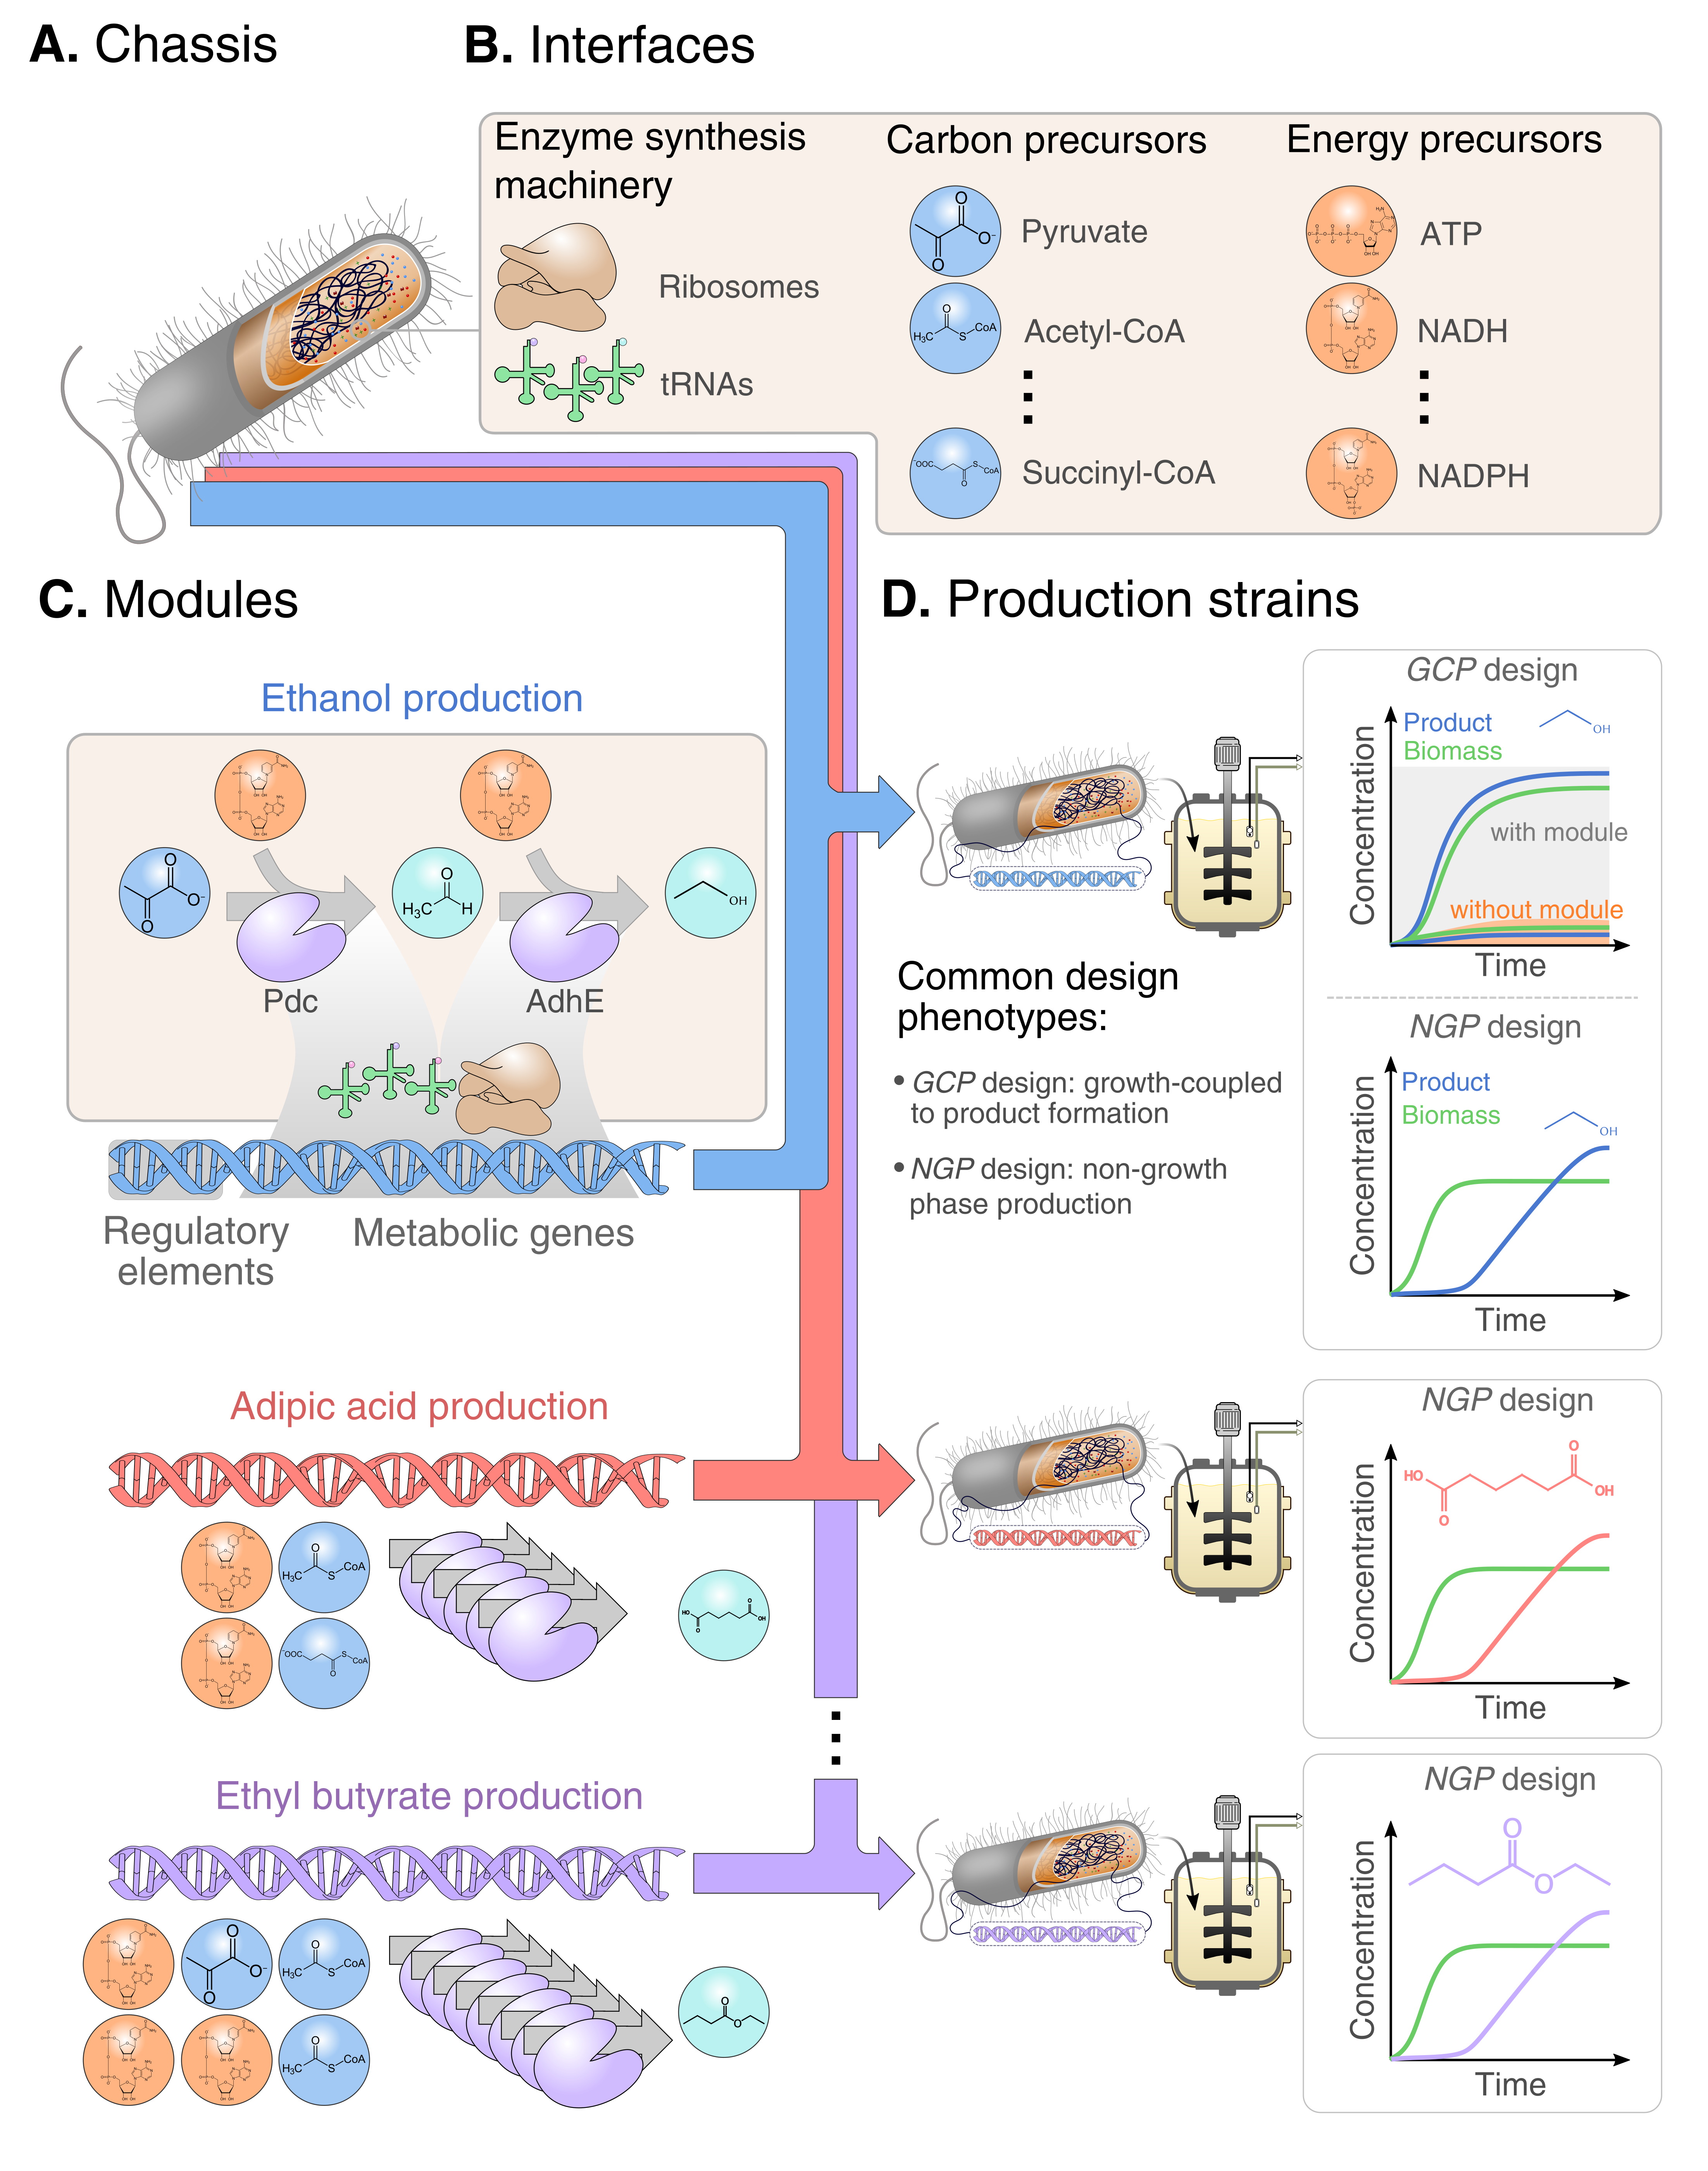
\includegraphics[width=\textwidth]{ba-fig3}
    \caption[Generalized concept of modular cell design]{Generalized concept of modular cell design.
    (\textbf{A}) Modular (chassis) cell. \textbf{(B)} Interfaces.
(\textbf{C}) Production modules. \textbf{(D)} Production strains. A
modular cell is designed to provide the necessary precursors for
biosynthesis pathway modules that are independently assembled with the
modular cell to generate production strains exhibiting desirable
phenotypes.}
    \label{fig:ba-fig3}
\end{figure}

\begin{figure}[h]
  \centering
  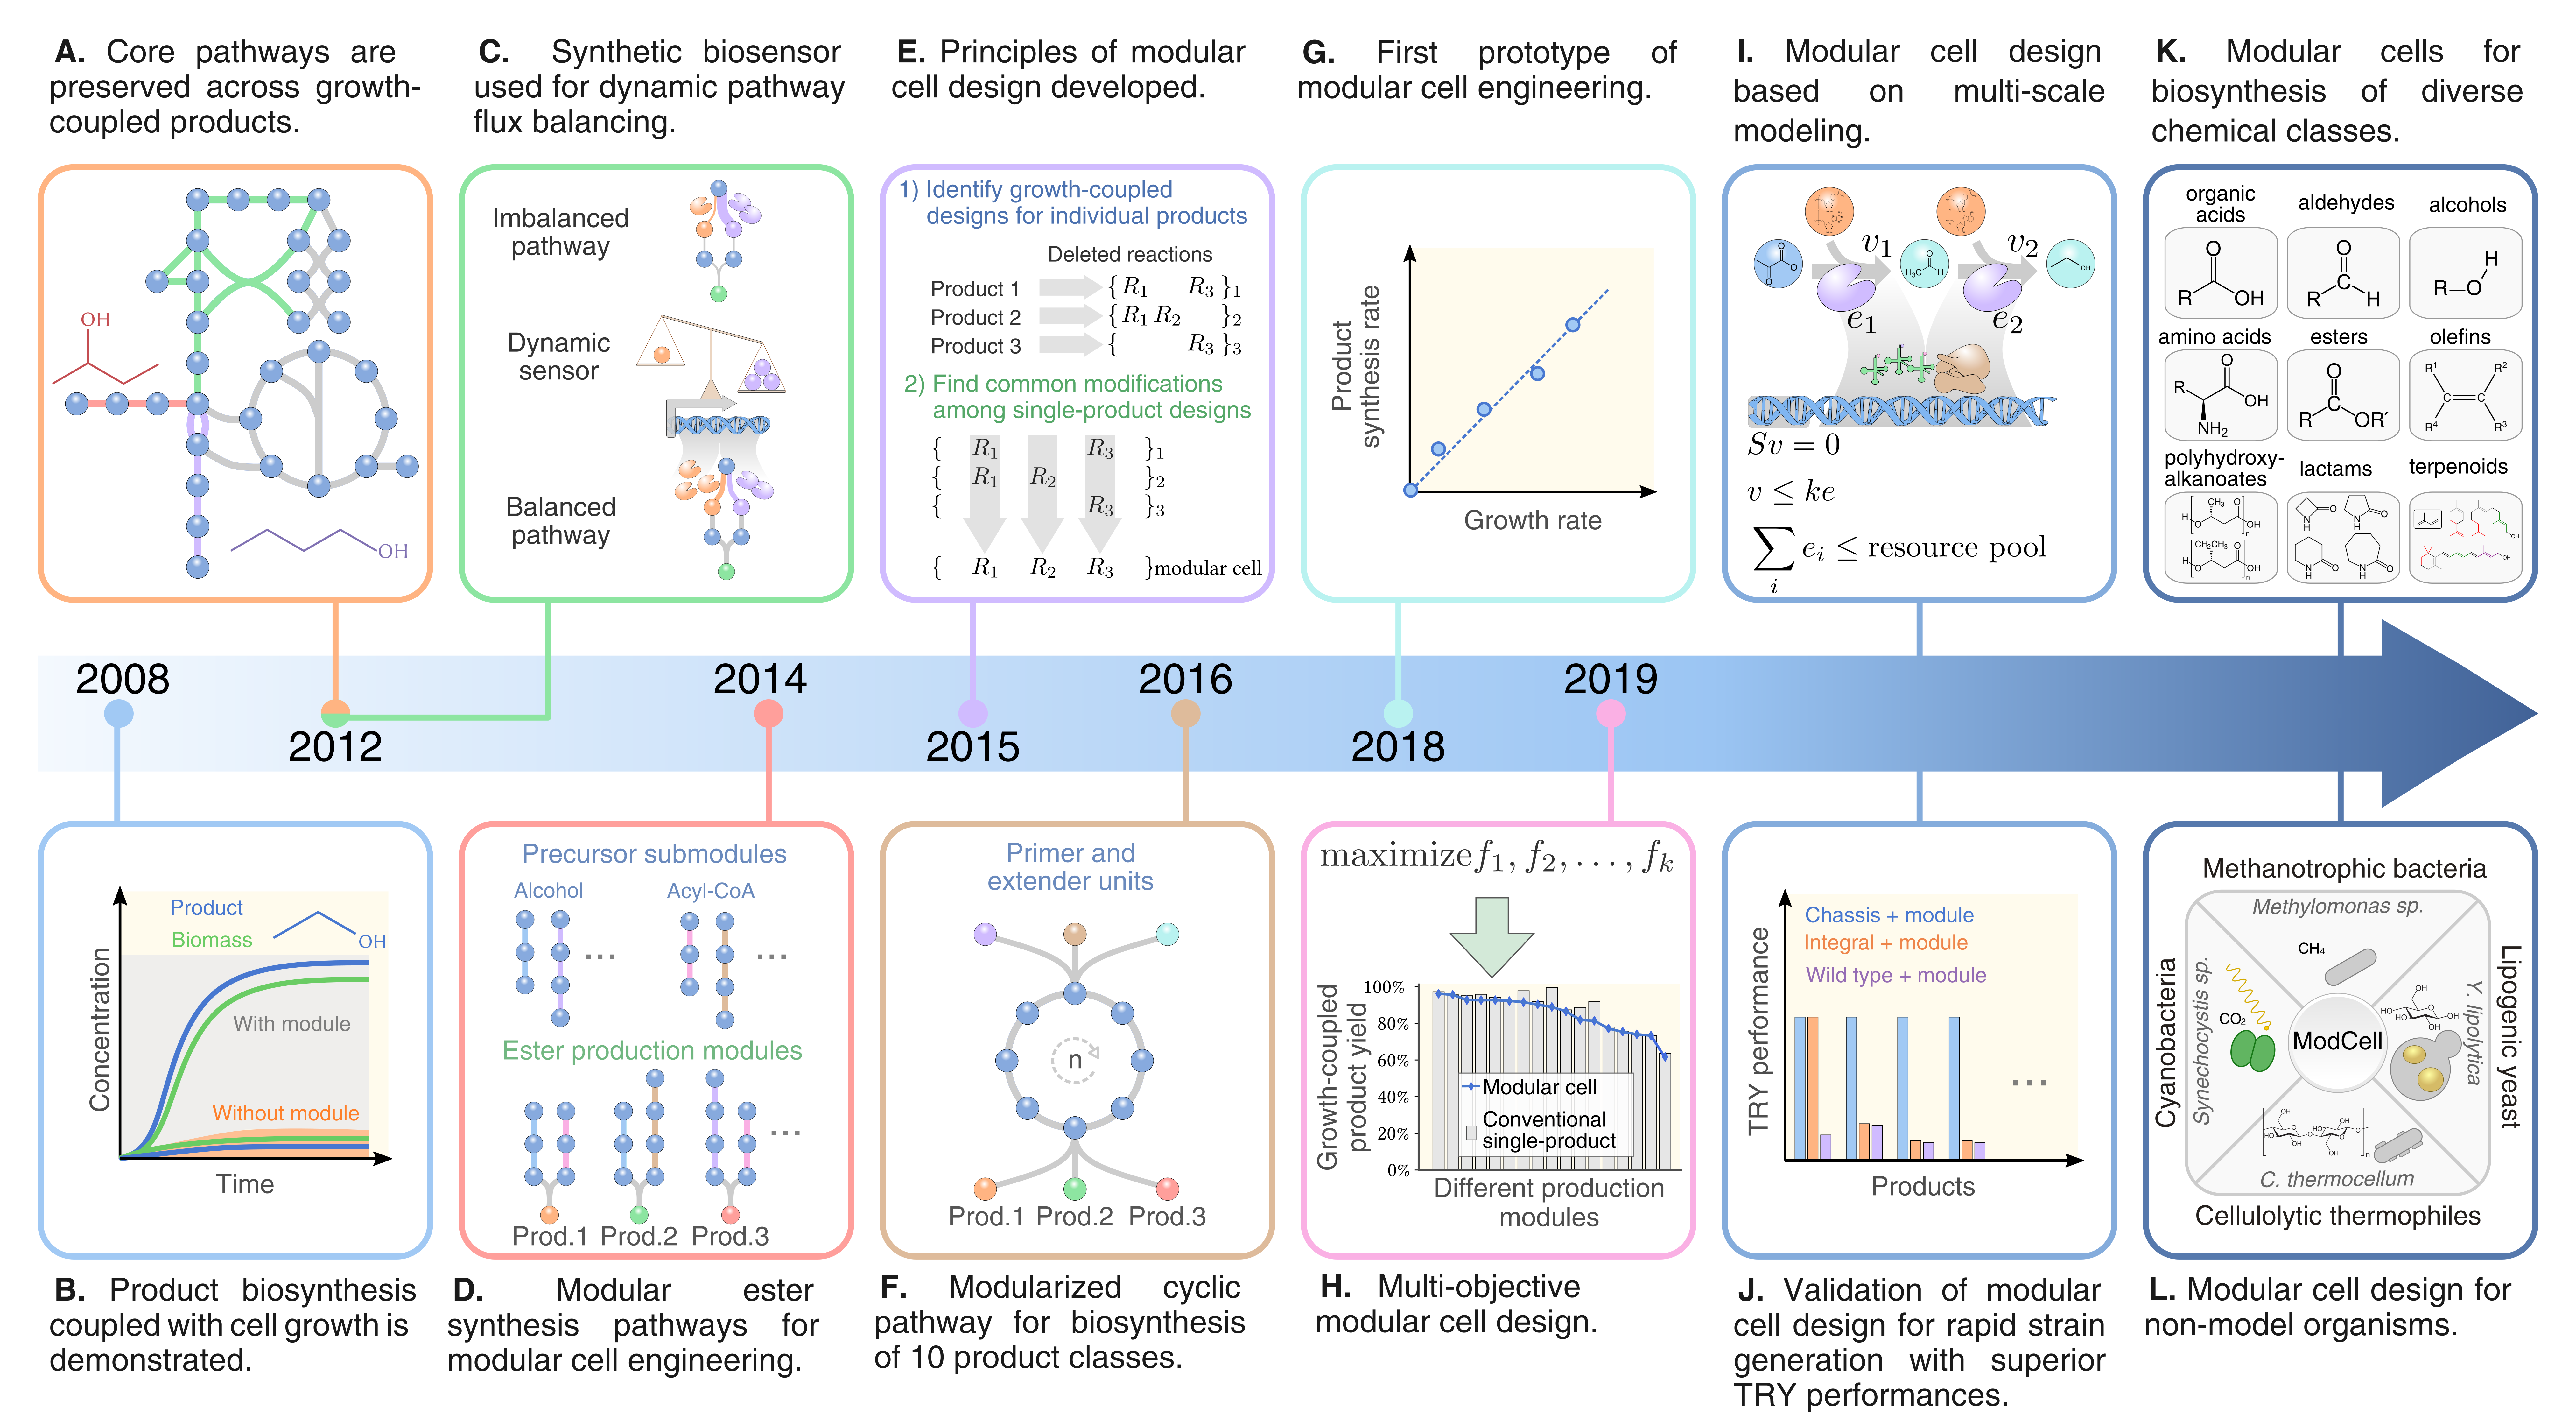
\includegraphics[width=\textwidth]{ba-fig4}
    \caption[Key advances and opportunities in the design and
    implementation of modular cells and exchangeable production modules]{Key advances and opportunities in the design and
implementation of modular cells and exchangeable production modules.
    (\textbf{A}) The same core metabolic pathways were revealed for butanol
and isobutanol growth-coupled production based on elementary mode
analysis \citep{trinh2012}. (\textbf{B}) An \emph{E. coli}
cell with minimal metabolic functionality designed to require product
(ethanol) synthesis for cell growth was experimentally validated
\citep{trinh2008}. (\textbf{C}) A dynamic sensor-regulator
system was designed and implemented to balance metabolic fluxes for
enhanced biosynthesis of fatty acid-derived molecules
\citep{zhang2012}. (\textbf{D}) A modular ester fermentative
pathway platform derived from alcohol and acyl-CoA pathway submodules
was designed and experimentally demonstrated in a chassis strain
\citep{layton2014}. (\textbf{E}) First modular cell design
method, named MODCELL, was proposed and used to design 3 modular cells
for the production of a group of alcohols and derived esters
\citep{trinh2015}. (\textbf{F}). Carbon and energy efficient
cyclic pathway was developed to synthesize 10 product classes from a
variety of primer and extender precursors \citep{cheong2016}.
(\textbf{G}) Prototypes of modular cell engineering were demonstrated
for growth-coupled to product synthesis predicted by MODCELL
\citep{trinh2015} and pathway optimization by adaptive
laboratory evolution \citep{wilbanks2017}. (\textbf{H})
Multi-objective optimization-based modular cell design method, named
ModCell2, will be developed in Chapter~\ref{ch:ms1} and used to reveal negligible trade-offs
between modular and integral designs.
(\textbf{I}) Next-generation of modular cell design framework is
proposed to account for enzyme biosynthesis cost using metabolism and
expression (ME) or kinetic models with enzyme constraints. (\textbf{J})
Experimental demonstration of rapid and systematic generation of modular
production strains with many different types of production modules to
achieve superior performances over the wildtype and single-product
(integral) strains in terms of titer, rate, and yield (TRY).
(\textbf{K}) Design of a universal modular cell compatible with a large
and diverse space of production modules. (\textbf{L}) Future
demonstration of modular cell design is proposed for
industrially-relevant, non-model organisms with difficult-to-transfer
phenotypes, such as efficient assimilation of CO\textsubscript{2},
    CH\textsubscript{4}, or cellulose.}
    \label{fig:ba-fig4}
\end{figure}


